\chapter{World of Warcraft (WoW) Features in MIA} \label{WoW}
\pagestyle{fancy}

\section{WoW Fishbot} \label{WoWFishbot}

\begin{note}
	As of World of Warcraft (WoW) version 7.2, this fishbot is fully functional.
\end{note}

The World of Warcraft (WoW) fishbot implementation within MIA was created solely for educational purposes. This fishbot violates the terms of use of WoW and should only be used at your own risk. The fishbot is designed to simulate fishing for ones character in WoW. 

\subsection{Setup and Configuration}

Before running the fishbot, there are a few things that need to be properly configured, otherwise the bot will either not work or not work efficiently. First, one must disable the hardware cursor in the system settings. This can be done by pressing escape, system, advanced, then setting hardware cursor to disable (see figure \ref{hardwar cursor}). Be sure to click apply before closing out of the settings.

\begin{lstlisting}
ESC > System > Advanced > Hardware Cursor > DISABLE > Apply
\end{lstlisting}

\begin{figure}[h]
	\centering
	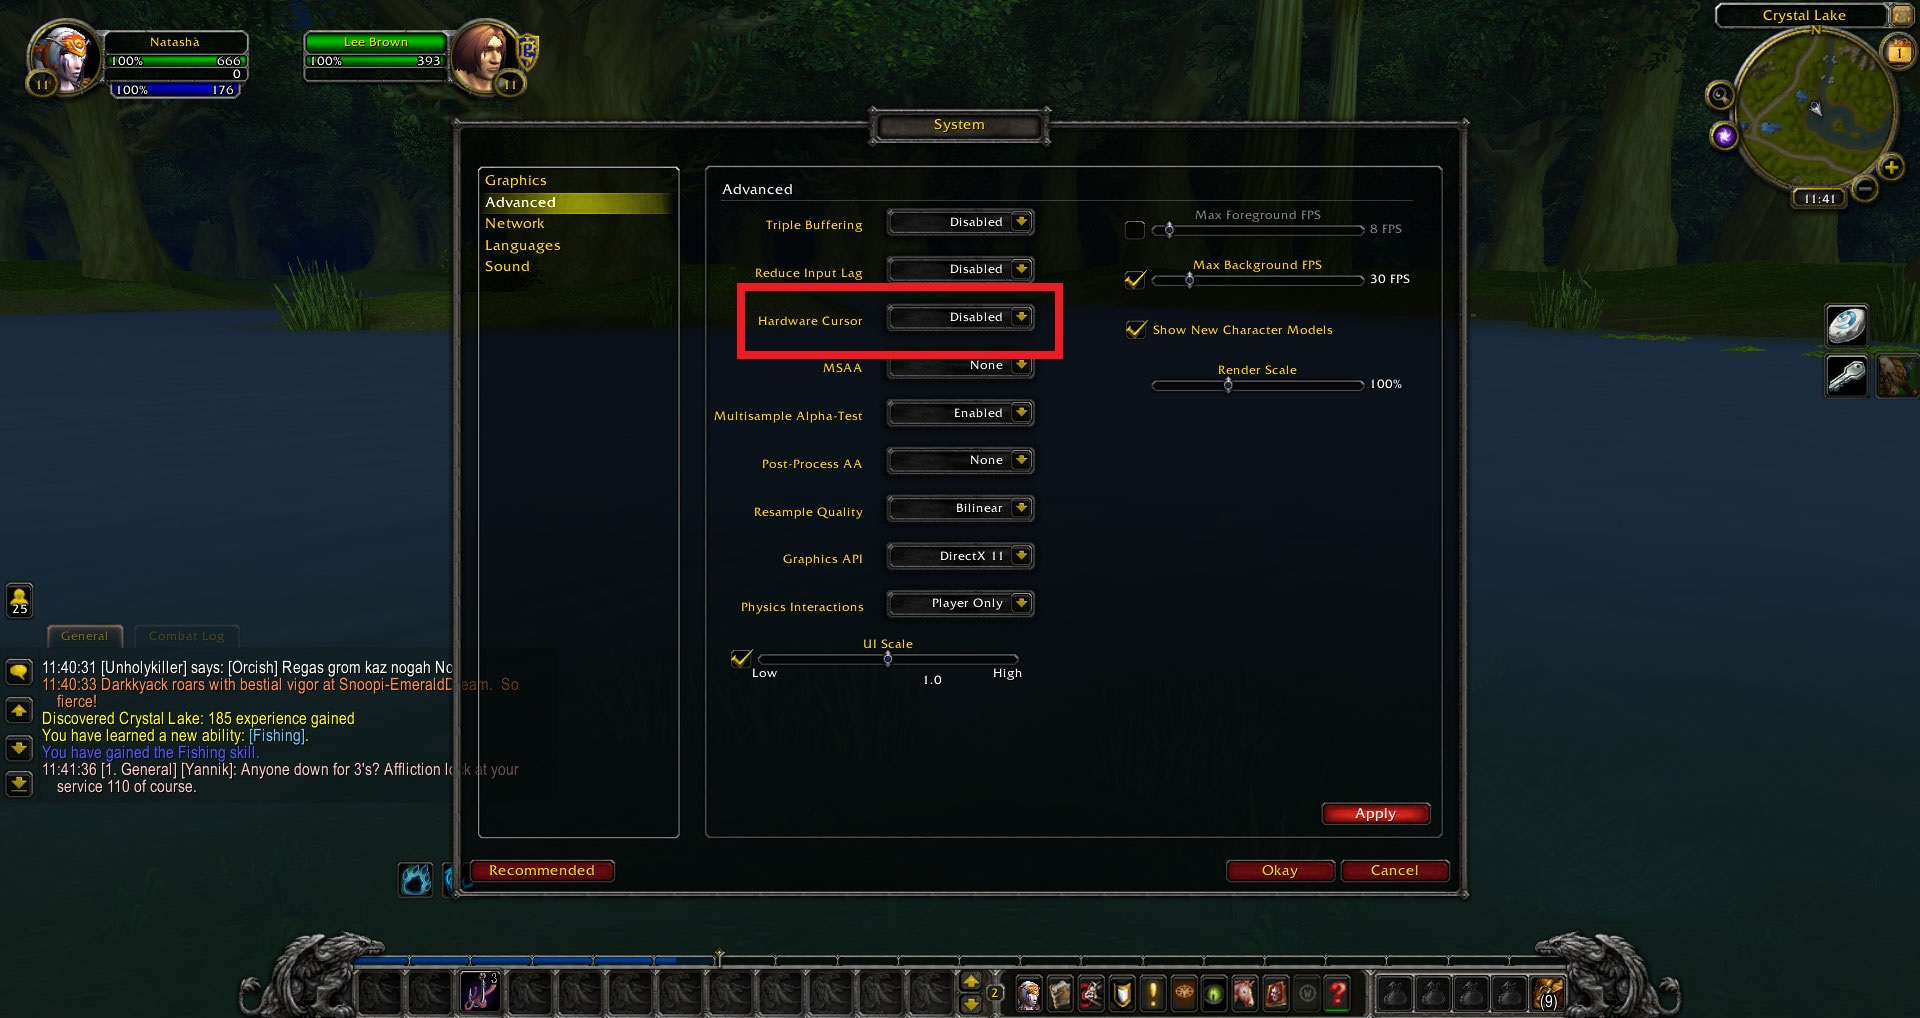
\includegraphics[width=0.9\textwidth]{Images/WoWScrnShot_040118_234154.jpg}
	\caption{Visual representation of the location of the option for disabling the hardware cursor. In order for the WoW fishbot to work, this option must be disabled.} \label{hardwar cursor}
\end{figure}

After disabling the hardware cursor, the coordinates for cast locations need to be set. It is recommended that the user zoom into first person when using the fishbot though this is not required for functionality. First, place the cast button on the action bar (see figure \ref{cast bar}). By default, the fishbot uses button 3 for cast, but upon running the fishbot the user will be prompted to change the settings. Similarly, a lure can be added to the bar, which by default is placed in action bar slot 8. A lure is optional and the fishbot program will ask if one is being used upon runtime.

\begin{figure}[h]
	\centering
	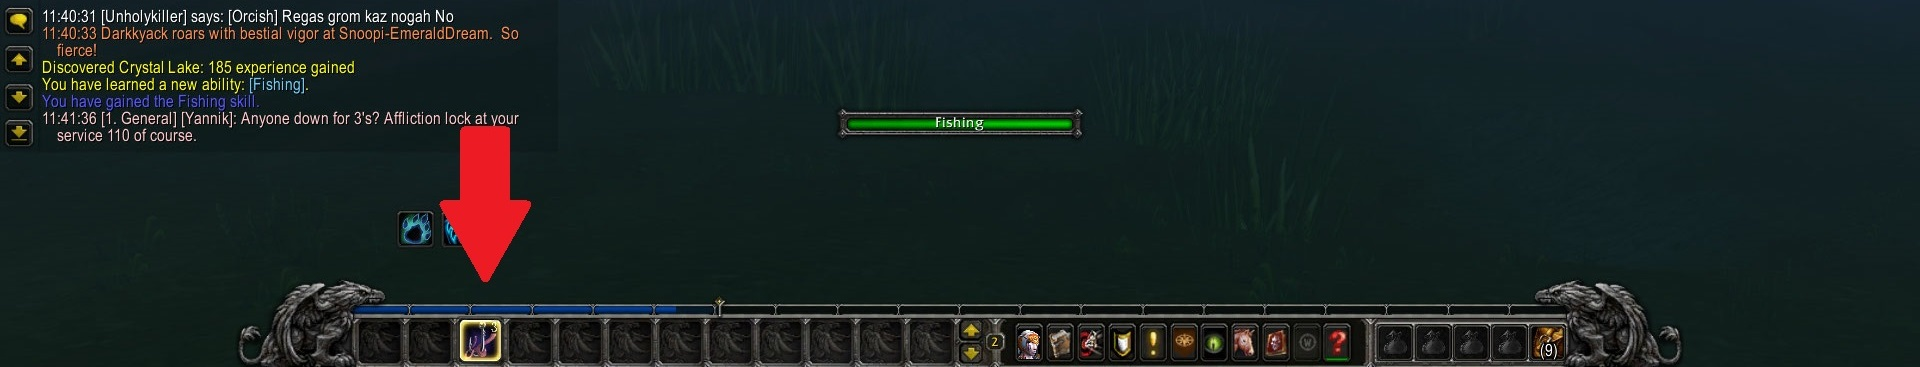
\includegraphics[width=0.9\textwidth]{Images/WoWScrnShot_040118_234212.jpg}
	\caption{Visual representation of the location of the cast option on the action bar.} \label{cast bar}
\end{figure}

The MIAC contains four separate variables that will most likely need to be configured for each user for use with the fishbot. The default values were set based on the creators environment and are not guaranteed to work for everyone. The options and their default values (at the time of writing this) are listed below.

\begin{lstlisting}
# Variables relating to the fishbot implementation inside MIA.
WoWFishBotStartX=725
WoWFishBotStartY=360
WoWFishBotEndX=1230
WoWFishBotEndY=495
\end{lstlisting}

\begin{figure}[h]
	\centering
	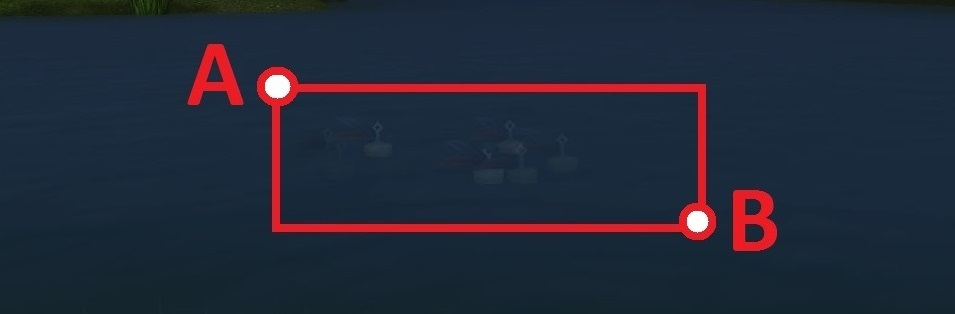
\includegraphics[width=0.8\textwidth]{Images/WoWScrnShot_040118_234212b.jpg}
	\caption{The red square represents the region in which the casted bobber lands. The two points labeled A and B are positions that one would want to set as the proper coordinates in the MIAC (see section \ref{MIAC} for more details).} \label{fishbot square}
\end{figure}

These values, \inlinecode{WoWFishBotStartX, WoWFishBotStartY, WoWFishBotEndX, WoWFishBotEndY}, define the area that the fishbot will search for the fish bobber within. The first two parameters, \inlinecode{WoWFishBotStartX, WoWFishBotStartY} define the coordinates of the point A in figure \ref{fishbot square}. The second two parameters, \inlinecode{WoWFishBotEndX, WoWFishBotEndY} define the coordinates of the point B in figure \ref{fishbot square}. The MIA fishbot will search this area for the bobber during operation. The best method to determine the proper coordinates to use is to spam the cast option and observe the area that the bobber lands. The suggested coordinates for A and B are near where they are located in figure \ref{fishbot square}, however any coordinates can be used. To determine the proper coordinates, one can use the \inlinecode{find mouse} command in MIA which will determine the coordinates at the location of ones cursor.

After these parameters are set, the fishbot can be run in MIA by using the \inlinecode{fishbot} command. There are a few other variables and parameters that can be set by the user but the others are optional. These other optional parameters that are contained in the MIAC are as follows.

\begin{lstlisting}
# Variables relating to the fishbot implementation inside MIA.
WoWFishBotIncrement=40
WoWFishBotNumOfCasts=10000
WoWFishBotDelay=10000
\end{lstlisting}

First, the \inlinecode{WoWFishBotIncrement} variable defines the step size that the MIA program will search for the bobber by. This can be seen in figure \label{fishbot increments}. A smaller step size will cause the fishbot to find the bobber slower but more accurate, whereas a faster step size will cause a faster search but is less accurate. The default value for this is 40, but should be decreased if the bobber is missed by the fishbot. The next parameter, \inlinecode{WoWFishBotNumOfCasts} is how many times the fishbot will cast before ending it's program. This can be whatever the user desires. 



\begin{figure}[h]
	\centering
	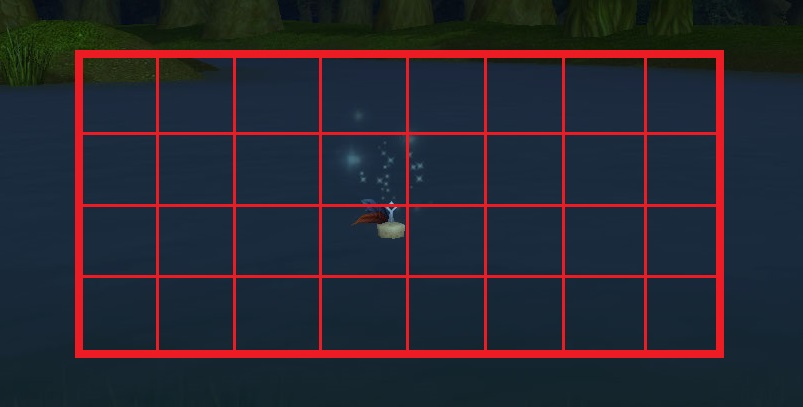
\includegraphics[width=0.8\textwidth]{Images/WoWScrnShot_040118_234227b.jpg}
	\caption{The red square similar to that shown in figure \ref{fishbot square} partitioned into squares of size defined by the \inlinecode{WoWFishBotIncrement} value.} \label{fishbot increments}
\end{figure}

\begin{figure}[h]
	\centering
	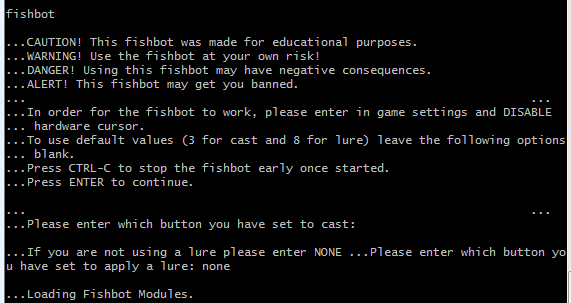
\includegraphics[width=0.7\textwidth]{Images/fishbot_MIA.png}
	\caption{A snapshot of the MIA fishbot upon runtime. As of MIA version 0.041.} \label{fishbot terminal}
\end{figure}

The last parameter, \inlinecode{WoWFishBotDelay} is what defines how fish are caught. The MIA fishbot catches fish by chance. There is a plan to improve the method to catch fish by, but for now the program waits a specific number of milliseconds after finding the bobber before clicking it. Thus, there is a certain probability that a fish is caught. By default this value is 10000ms.

To run the fishbot simply use the \inlinecode{fishbot} command in the MIA terminal. Upon running this command, the fishbot will ask the use to enter the required information (see figure \ref{fishbot terminal})

\section{Mailbox Management} \label{WoWMailbox}

MIA contains some in game mail management for World of Warcraft (WoW) in order to assist in the process of creating in game letters in bulk. In game letters can't be sent between characters and then looted and stored in the character inventories. In some cases, such as role playing (RP) or guild recruitment, these letters may be desired by bulk. The process of creating these letters consists of entering in a letter recipient, subject, the contents of the letter, and then hitting a send button (see figure \ref{wow mailbox send}). After sending these letters, however many times it is done, they then need to be looted on the character that they were sent to. This consists of opening up the mailbox, clicking on the letter received, acquiring hte physical copy by looting it from the opened letter, then deleting the letter to clean up the mailbox (see figure \ref{wow mailbox receive}). MIA is designed to automate this entire process.

\subsection{Sending Duplicates of a Letter}

As described above briefly, MIA has the capability of automating the sending of duplicate letters to a recipient in WoW. To do this, there are a few settings that need to be configured on the user end to ensure proper functionality. There are two variables contained in the MIAC (see section \ref{MIAC} for more information) that are used in conjunction with the \inlinecode{wow dup letter} function in MIA. These are listed below.

\begin{lstlisting}
# WoW related variables.
WoWMailboxSendLetterLocationX=279
WoWMailboxSendLetterLocationY=647
\end{lstlisting}

By default, these values are set for the environment that was used when originally programmed into MIA. Both of these variables are used to represent the location of the send button shown in figure \ref{wow mailbox send}. The first, \inlinecode{WoWMailboxSendLetterLocationX} represents the x coordinate and the latter \inlinecode{WoWMailboxSendLetterLocationY} represents the y coordinate. Both of these values can be found by using the \inlinecode{find mouse} function in MIA. 

\begin{figure}[h]
	\centering
	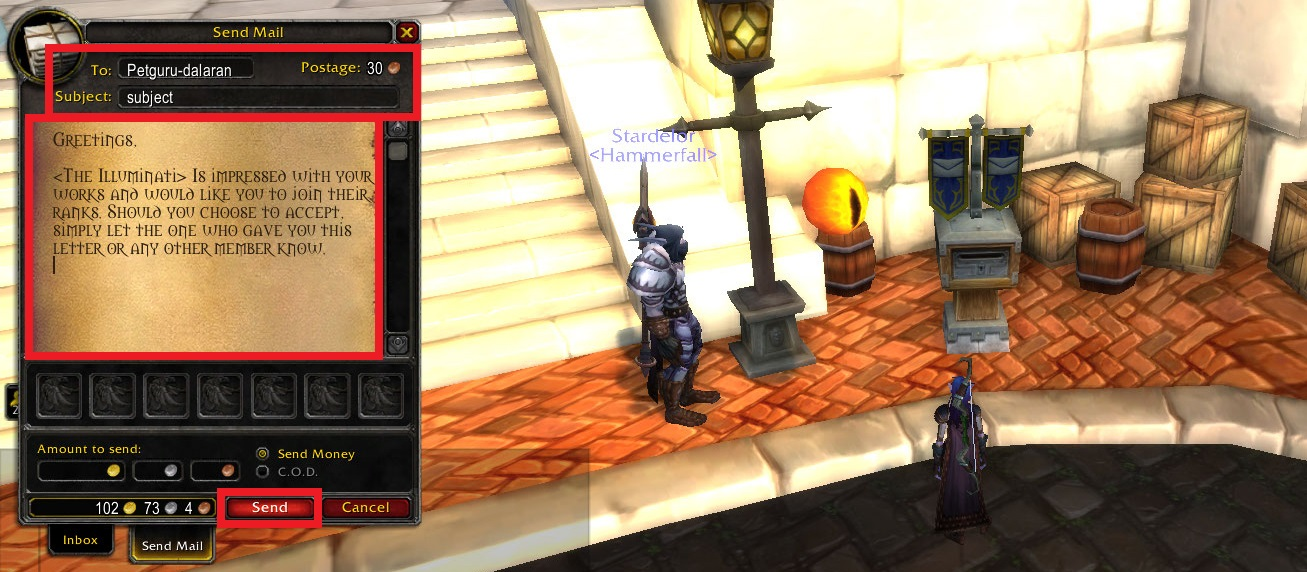
\includegraphics[width=0.9\textwidth]{Images/WoWScrnShot_040518_181350b.jpg}
	\caption{A screen shot of the WoW in game outgoing mailbox menu. The mail management within MIA utilizes the fields indicated by red squares in this menu. The red box around the send button represents the \inlinecode{WoWMailboxSendLetterLocation} location.} \label{wow mailbox send}
\end{figure}

Once the proper coordinates are set, one can automate this process of sending a duplicate letter by using the \inlinecode{wow dup letter} command in the MIA terminal. The \inlinecode{wow dup letter} has a few limitations when used. First, the recipient of the letter can only contain normal characters such as a, e, o, etc. The recipient cannot contain special characters such as \"{a}, \'{e}, \~{o}, etc. However, the contents of the message that will be sent can contain special characters. The desired message contents should be copied to the clipboard before running the \inlinecode{wow dup letter} command. Upon running the command, the terminal will prompt the user to do so as well. The subject field will automatically be filled in with "subject."

\begin{figure}[h]
	\centering
	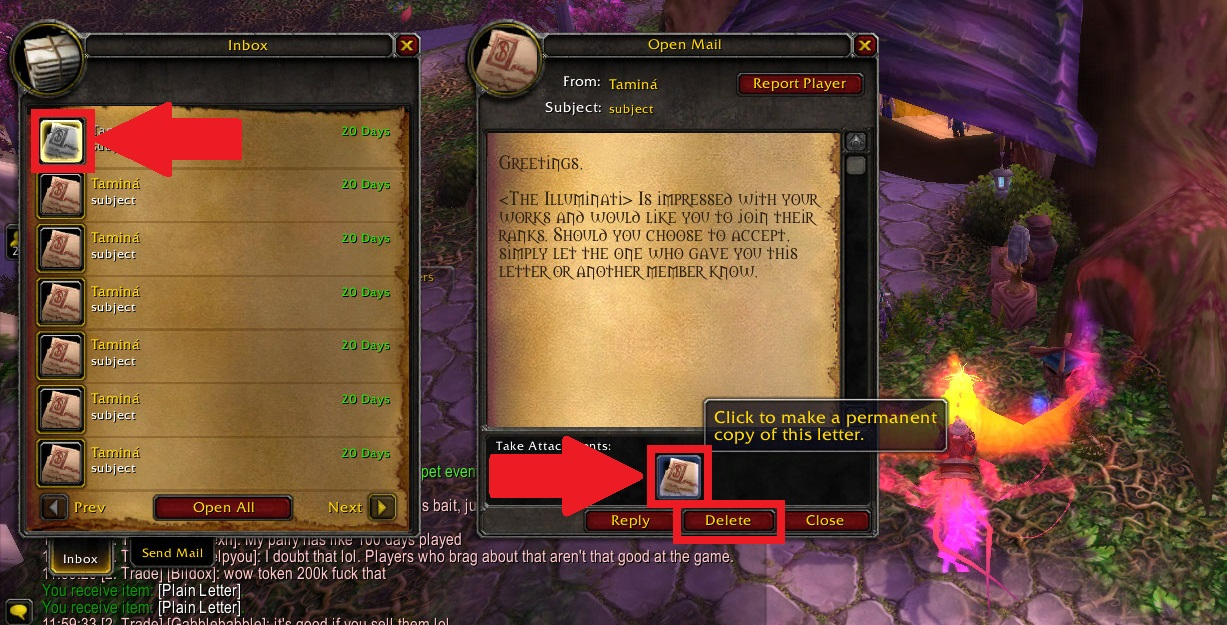
\includegraphics[width=0.9\textwidth]{Images/WoWScrnShot_040518_115947b.jpg}
	\caption{A screen shot of the WoW in game incoming mailbox menu. The mail management within MIA utilizes the fields indicated by red squares in this menu. The left arrow indicates the \inlinecode{WoWMailboxFirstLetterLocation} position. The right arrow indicates the \inlinecode{WoWMailboxLootLetterLocation} position. The square around the delete button represents the \inlinecode{WoWMailboxDeleteLetterLocation} location.} \label{wow mailbox receive}
\end{figure}

\subsection{Unloading Duplicated letters}

MIA contains a command \inlinecode{wow unload} which is designed to be used in conjunction with the \inlinecode{wow dup letter} command. This command will loot the letters from the incoming mailbox that are sent using the \inlinecode{wow dup letter} command. In order to use this command properly, there are six different variables within the MIAC that need to be determined for the users environment. These variables are below.

\begin{lstlisting}
# WoW related variables.
WoWMailboxFirstLetterLocationX=55
WoWMailboxFirstLetterLocationY=265
WoWMailboxLootLetterLocationX=675
WoWMailboxLootLetterLocationY=600
WoWMailboxDeleteLetterLocationX=700
WoWMailboxDeleteLetterLocationY=650
\end{lstlisting}

By default, these variables are set to values that were specific to the programmers environment. The variables need to be set based off of three different coorindates. The first, \inlinecode{WoWMailboxFirstLetterLocation} corresponds to the location of the first letter in the inbox of the user (see figure \ref{wow mailbox receive}). The second, \inlinecode{WoWMailboxLootLetterLocation} corresponds to the location of the letter to loot from the user inbox (see figure \ref{wow mailbox receive}). The last, \inlinecode{WoWMailboxDeleteLetterLocation} represents the locations of the delete button on a letter in the WoW inbox (see figure \ref{wow mailbox receive}).  For all three coordinates, there is an x and y value (represented by the variables in the MIAC) which can be determined through MIA by using the \inlinecode{find mouse} command.